\documentclass[aspectratio=169, 10pt]{beamer} 
% aspectratio=169 fuerza el formato panorámico

% --- TEMA Y FUENTES ---
\usetheme{metropolis}
% Opciones del tema: Bloques con fondo de color y barra de progreso
\metroset{block=fill, progressbar=frametitle, background=light}

\usepackage[sfdefault]{raleway} % Fuente moderna sans-serif
\usepackage[T1]{fontenc}
\usepackage[utf8]{inputenc}
\usepackage[spanish]{babel}

% --- PAQUETES GRÁFICOS ---
\usepackage{graphicx}
\usepackage{booktabs}
\usepackage{tikz}
\usetikzlibrary{positioning, arrows.meta, shapes, calc, shadows, decorations.pathmorphing, patterns, fit, backgrounds}
\usepackage{fontawesome5} % Para iconos modernos

% --- COLORES PERSONALIZADOS ---
\definecolor{primary}{RGB}{0,102,204}      % Azul corporativo
\definecolor{secondary}{RGB}{51,153,255}    % Azul claro
\definecolor{accent}{RGB}{255,87,34}        % Naranja acento
\definecolor{darkgray}{RGB}{60,60,60}
\definecolor{success}{RGB}{76,175,80}       % Verde éxito
\definecolor{warning}{RGB}{255,152,0}       % Amarillo advertencia
\definecolor{trafocolor}{RGB}{65,90,119}       % Violeta transformador
\definecolor{compcolor}{RGB}{2,62,138}        % Azul compensador

% Asignación de colores al tema
\setbeamercolor{palette primary}{bg=primary, fg=white}
\setbeamercolor{frametitle}{bg=primary, fg=white}
\setbeamercolor{alerted text}{fg=accent}
\setbeamercolor{progress bar}{fg=accent, bg=primary!30}

% --- PIE DE PÁGINA ---
\setbeamertemplate{footline}{
    \begin{beamercolorbox}[wd=\paperwidth, ht=3ex, dp=1.2ex, leftskip=1em, rightskip=1em]{footline}
        \raisebox{-0.7ex}{\includegraphics[height=2.86ex]{logo_placeholder}}
        \hspace{0.5em}
        {\scriptsize\color{gray} -- ADCSE -- Transformadores de Estado Sólido}
        \hfill
        \insertframenumber{} / \inserttotalframenumber
    \end{beamercolorbox}
}

% --- INFORMACIÓN DE LA PRESENTACIÓN ---
\title{Transformadores de Estado Sólido (SST)}
\subtitle{Regulación de tensión y resiliencia mediante desacoplo activo}
\author{Felipe Agustín Cruelles García}
\institute{Análisis Dinámico y Control de Sistemas Eléctricos de Potencia}
\date{19 de febrero de 2026}

\begin{document}

% 1. PORTADA
\begin{frame}
    \titlepage
\end{frame}

% 2. ÍNDICE
\begin{frame}{Contenido}
    \setbeamertemplate{section in toc}[sections numbered]
    \tableofcontents
\end{frame}

% --- SECCIÓN 1 ---
\section{Introducción}

\begin{frame}{¿Qué vamos a ver hoy?}
    \begin{columns}[T]
        \column{0.5\textwidth}
        \vspace{0.5em}
        
        \begin{itemize}
            \item Una tendencia tecnológica \textbf{emergente} en el campo del control de tensión.
            \item Los \textbf{\textcolor{accent}{Transformadores de Estado Sólido (SST)}}.
            \item Conocidos como \textit{Solid State Transformers} en inglés.
        \end{itemize}
        
        \vspace{0.5em}
        \begin{alertblock}{Objetivo}
            Entender cómo esta tecnología revoluciona la distribución eléctrica.
        \end{alertblock}
        
        \column{0.5\textwidth}
        \centering
        \begin{tikzpicture}[scale=0.85, transform shape]
            % Caja principal del SST
            \draw[fill=secondary!20, draw=primary, line width=2pt, rounded corners] 
                (0,0) rectangle (4,3);
            \node[font=\Large\bfseries, primary] at (2,2.3) {SST};
            
            % Bus DC (centrado)
            \draw[accent, line width=2pt] (0.3,1.5) -- (3.7,1.5);
            \node[accent, font=\scriptsize] at (2,1.8) {Bus DC};
            
            % Etapas internas (centradas debajo del Bus DC)
            \draw[fill=white, draw=primary] (0.3,0.3) rectangle (1.3,1.1);
            \node[font=\scriptsize] at (0.8,0.7) {AC/DC};
            
            \draw[fill=white, draw=primary] (1.5,0.3) rectangle (2.5,1.1);
            \node[font=\scriptsize] at (2.0,0.7) {DC/DC};
            
            \draw[fill=white, draw=primary] (2.7,0.3) rectangle (3.7,1.1);
            \node[font=\scriptsize] at (3.2,0.7) {DC/AC};
            
            % Conexiones
            \draw[-Stealth, thick] (-1,1.5) -- (0,1.5) node[midway, above, font=\scriptsize] {MT};
            \draw[-Stealth, thick] (4,1.5) -- (5,1.5) node[midway, above, font=\scriptsize] {BT};
        \end{tikzpicture}
    \end{columns}
\end{frame}

% --- SECCIÓN 2 ---
\section{Conceptos Previos}

\begin{frame}{Recordatorio 1: Transformador Convencional}
    \begin{columns}
        \column{0.5\textwidth}
        \textbf{¿Qué hace?}
        \begin{itemize}
            \item Transforma niveles de tensión en CA.
            \item Utiliza campos electromagnéticos.
            \item Dos devanados acoplados magnéticamente.
        \end{itemize}
        
        \vspace{0.5em}
        \textbf{Importancia:}
        \begin{itemize}
            \item Razón principal del uso de corriente alterna.
            \item Eficiencia energética en transmisión.
        \end{itemize}

        \column{0.5\textwidth}
        \centering
        % Imagen del transformador convencional
        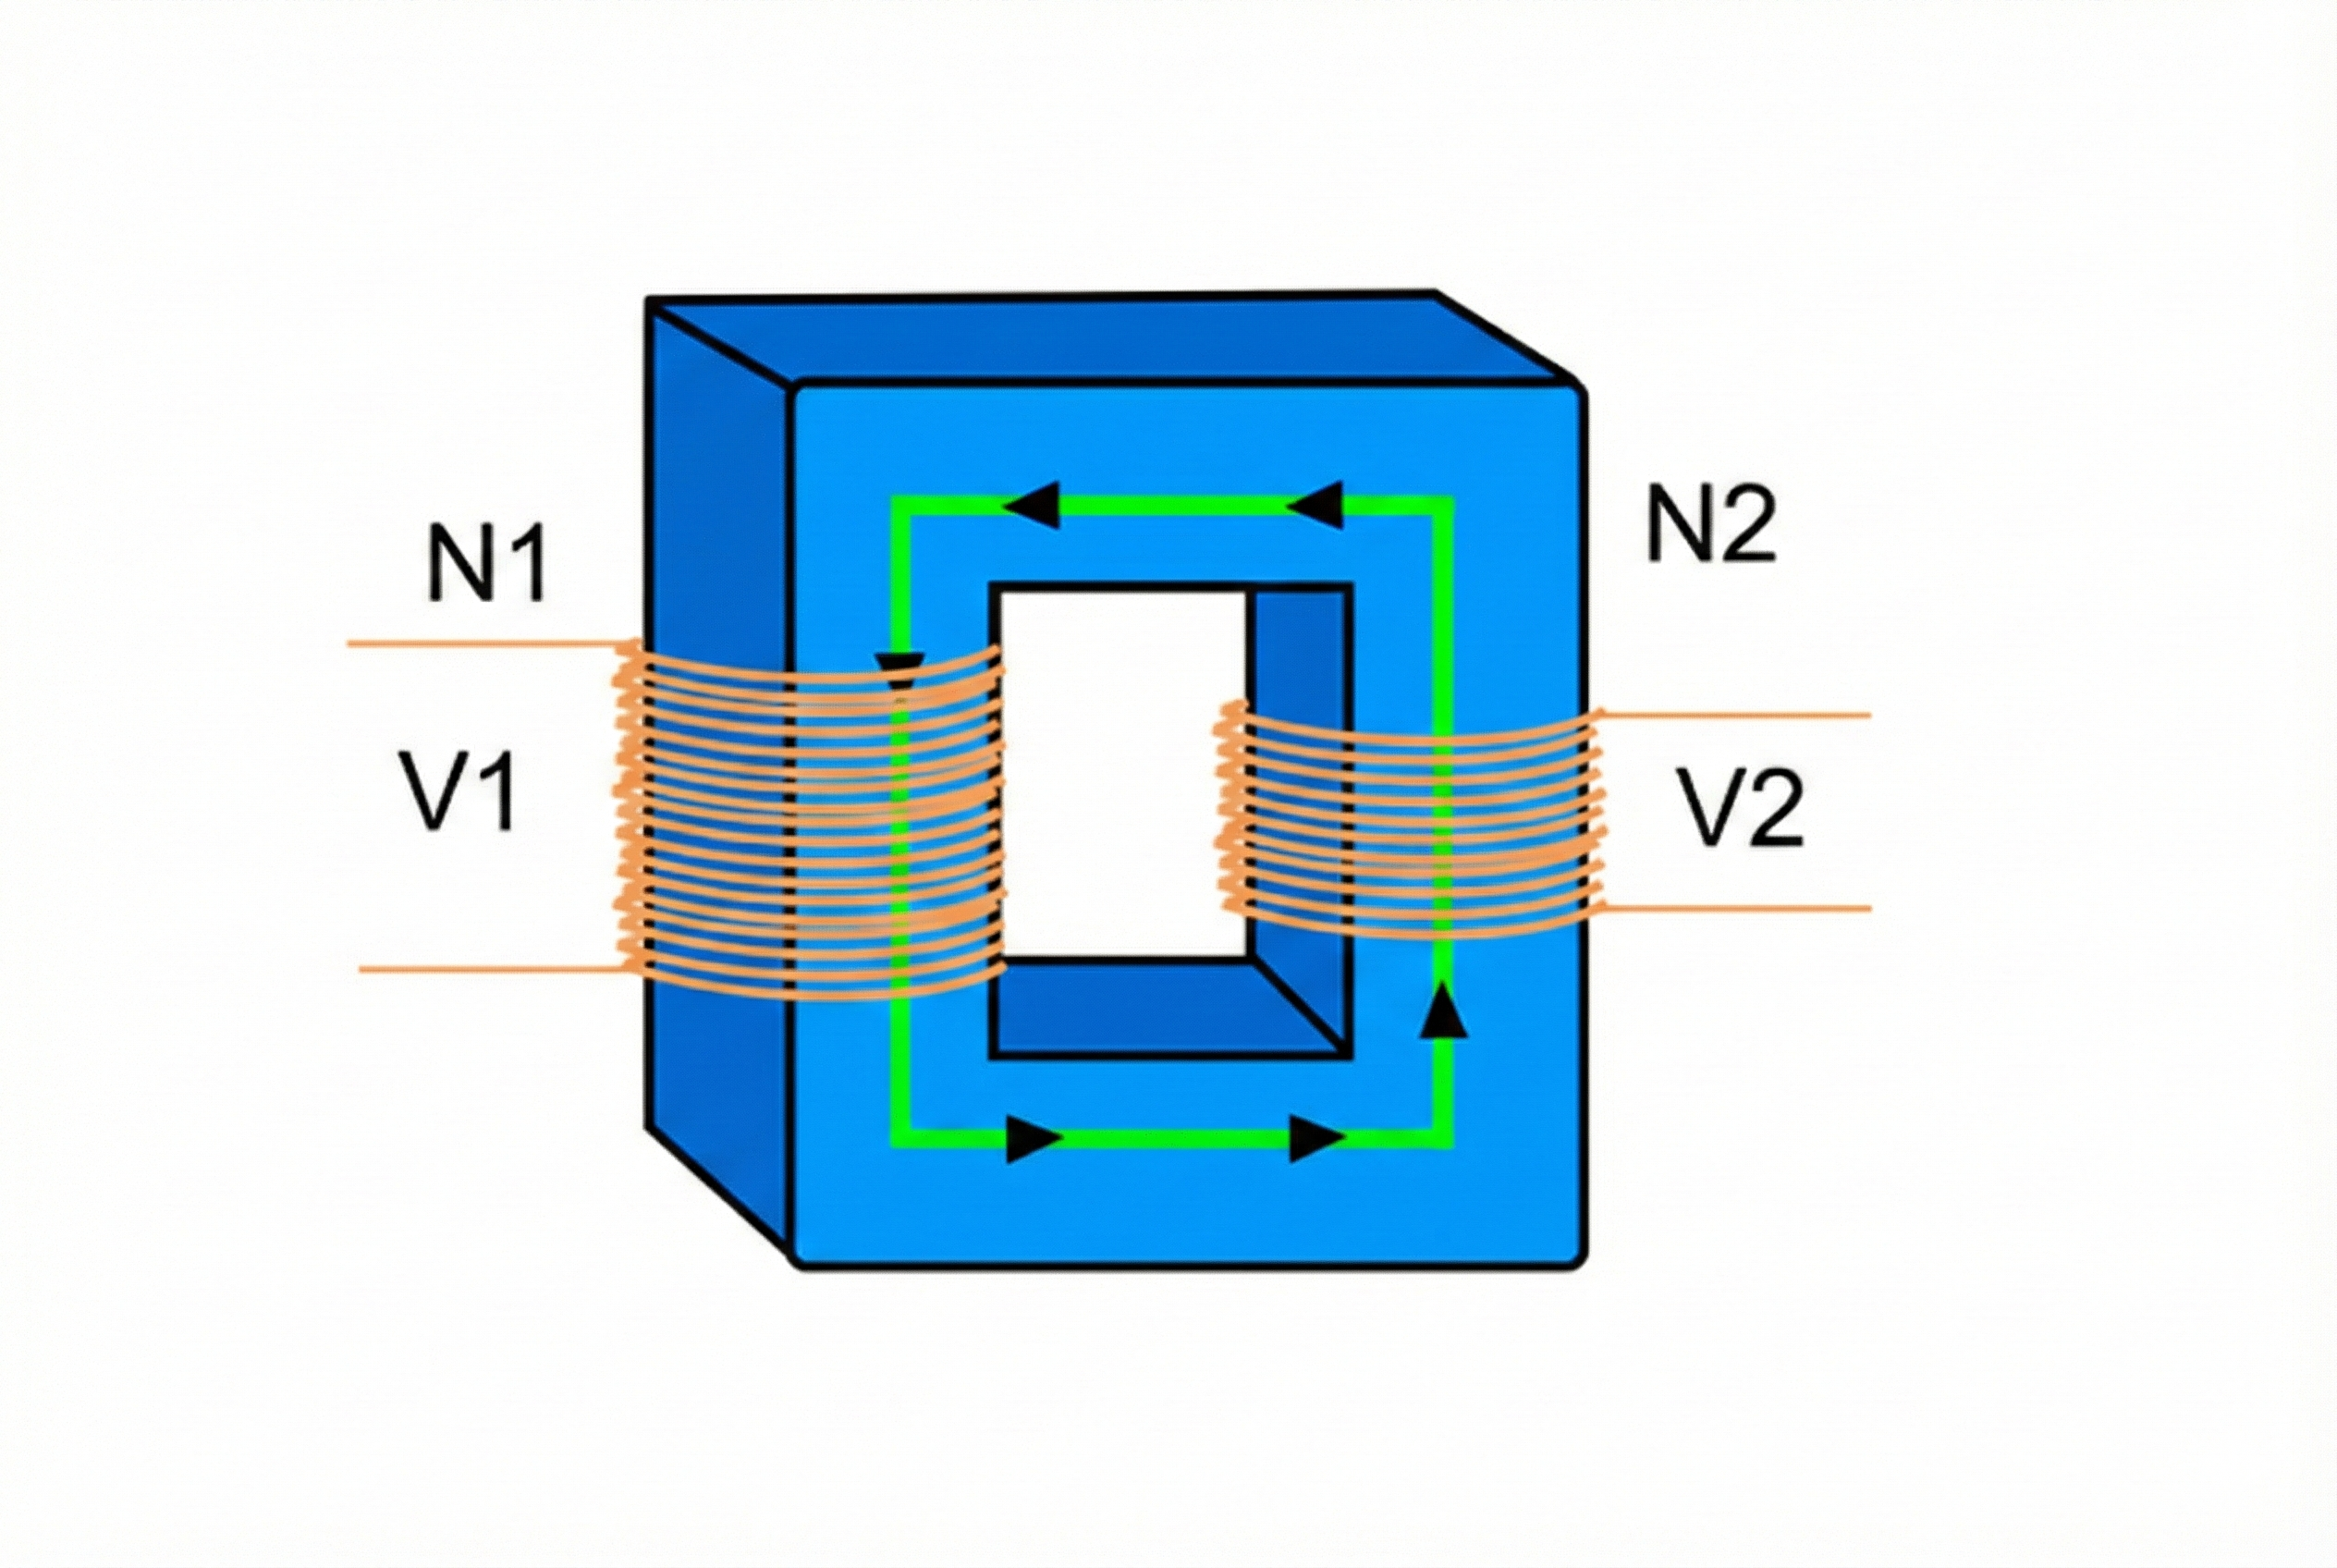
\includegraphics[width=0.9\linewidth]{trafo_convencional.png}
        
        \vspace{0.3em}
        \[
            \frac{V_1}{V_2} = \frac{N_1}{N_2}
        \]
    \end{columns}
\end{frame}

\begin{frame}{Recordatorio 2: STATCOM}
    \begin{columns}
        \column{0.55\textwidth}
        \textbf{Función principal:}
        \begin{itemize}
            \item Control de tensión en la red.
            \item Mejora calidad del suministro.
            \item Intercambio de potencia reactiva.
        \end{itemize}
        
        \vspace{0.5em}
        \textbf{Características:}
        \begin{itemize}
            \item Conexión en \textbf{\textcolor{accent}{paralelo}}.
            \item Basado en VSC (\textit{Voltage Source Converters}).
            \item Consume solo potencia activa para pérdidas.
        \end{itemize}

        \column{0.45\textwidth}
        \centering
        \begin{tikzpicture}[scale=0.85]
            % Red eléctrica (línea principal)
            \draw[line width=2pt] (-1,2) -- (4,2);
            \node[above, font=\small] at (1.5,2) {Nudo};
            
            % STATCOM conectado en paralelo
            \draw[primary, line width=2pt] (2,2) -- (2,0.2);
            \draw[fill=secondary!30, draw=primary, line width=1.5pt] 
                (0.8,0.2) rectangle (3.2,-1.5);
            
            % Texto STATCOM arriba, VSC abajo: sin solapamiento
            \node[font=\small\bfseries, primary] at (2,-0.3) {STATCOM};
            \node[font=\tiny, darkgray] at (2,-0.85) {(VSC)};
            
            % Flechas de potencia reactiva (colores coherentes con STATCOM)
            \draw[-Stealth, primary, line width=1.5pt] (2.6,1.8) -- (2.6,0.4);
            \draw[-Stealth, primary, line width=1.5pt] (1.4,0.4) -- (1.4,1.8);
            \node[font=\small, primary, text width=1.5cm, align=center] at (4.0,1) {$Q$ reactiva};
            
            % Tierra (símbolo estándar IEC)
            \draw[thick] (2,-1.5) -- (2,-2);
            \draw[thick] (1.4,-2) -- (2.6,-2);
            \draw[thick] (1.6,-2.2) -- (2.4,-2.2);
            \draw[thick] (1.8,-2.4) -- (2.2,-2.4);
        \end{tikzpicture}
        
        \vspace{0.3em}
        \begin{alertblock}{Clave}
            \centering Conexión en \textbf{derivación}
        \end{alertblock}
    \end{columns}
\end{frame}

% --- SECCIÓN 3 ---
\section{Transformadores de Estado Sólido}

\begin{frame}{¿Qué son los SST?}
    \begin{block}{Definición}
        Los SST son equipos de paso que se conectan \textbf{\textcolor{accent}{en serie}} al flujo de potencia, similar a los transformadores convencionales, pero usando electrónica de potencia.
    \end{block}

    \vspace{0.8em}

    \begin{center}
    \begin{tikzpicture}[auto, node distance=2.5cm, >=Stealth, scale=1.0, transform shape]
        % Red MT
        \node[circle, draw=primary, line width=2pt, minimum size=1cm, fill=white] (redMT) {};
        \draw[primary, line width=1.5pt] (redMT.north) -- ++(0,0.3);
        \draw[primary, line width=1.5pt] (redMT.south) -- ++(0,-0.3);
        \node[below=0.3cm of redMT, font=\small] {Red MT};
        
        % SST (sin subrectángulos que tapan el texto)
        \node[right=1.5cm of redMT, fill=secondary!30, draw=primary, line width=2pt, 
              minimum width=3cm, minimum height=1.5cm, rounded corners] (sst) {};
        \node[font=\Large\bfseries, primary] at (sst) {SST};
        
        % Red BT
        \node[circle, draw=primary, line width=2pt, minimum size=1cm, fill=white, right=1.5cm of sst] (redBT) {};
        \draw[primary, line width=1.5pt] (redBT.north) -- ++(0,0.3);
        \draw[primary, line width=1.5pt] (redBT.south) -- ++(0,-0.3);
        \node[below=0.3cm of redBT, font=\small] {Red BT};
        
        % Conexiones en serie
        \draw[very thick, primary, -Stealth] (redMT) -- (sst) node[midway, above, font=\scriptsize] {Serie};
        \draw[very thick, primary, -Stealth] (sst) -- (redBT) node[midway, above, font=\scriptsize] {Paso};
        
        % Comparación visual con STATCOM
        \node[below=1.2cm of sst, text width=10cm, align=center, font=\small] 
            {\textcolor{accent}{STATCOM} $\rightarrow$ Paralelo (Derivación) \quad vs. \quad \textcolor{primary}{SST} $\rightarrow$ Serie (Paso)};
    \end{tikzpicture}
    \end{center}
\end{frame}

\begin{frame}{Funcionalidad Híbrida}
    \begin{center}
        \begin{tikzpicture}
            % Ecuación visual
            \node[font=\Large, primary] (sst) at (0,0) {\textbf{SST}};
            \node[font=\Large] at (1.5,0) {=};
            
            % Transformador
            \node[draw=trafocolor, fill=trafocolor!15, rounded corners, minimum width=2.5cm, 
                  minimum height=1cm, line width=1.5pt] (trafo) at (3.8,0) {};
            \node[font=\small, trafocolor] at (trafo) {\textbf{Transformador}};

            \node[font=\Large] at (5.8,0) {+};

            % Compensador
            \node[draw=compcolor, fill=compcolor!15, rounded corners, minimum width=2.5cm, 
                  minimum height=1cm, line width=1.5pt] (comp) at (7.8,0) {};
            \node[font=\small, compcolor] at (comp) {\textbf{Compensador}};
        \end{tikzpicture}
    \end{center}

    \vspace{1.5em}

    \begin{columns}[t]
        \column{0.45\textwidth}
        {\setbeamercolor{block title example}{fg=white, bg=trafocolor}
        \setbeamercolor{block body example}{bg=trafocolor!10}
        \begin{exampleblock}{Como Transformador}
            \begin{itemize}
                \item[\textcolor{success}{\faCheckCircle}] Transforma tensión.
                \item[\textcolor{success}{\faCheckCircle}] Transfiere potencia activa.
                \item[\textcolor{success}{\faCheckCircle}] Aislamiento galvánico.
            \end{itemize}
        \end{exampleblock}}

        \column{0.45\textwidth}
        {\setbeamercolor{block title alerted}{fg=white, bg=compcolor}
        \setbeamercolor{block body alerted}{bg=compcolor!10}
        \begin{alertblock}{Como Compensador}
            \begin{itemize}
                \item[\textcolor{success}{\faCheckCircle}] Control de factor de potencia.
                \item[\textcolor{success}{\faCheckCircle}] Regulación dinámica.
                \item[\textcolor{success}{\faCheckCircle}] Eliminación de armónicos.
            \end{itemize}
        \end{alertblock}}
    \end{columns}
\end{frame}

% --- SECCIÓN 4 ---
\section{Características Principales}

\begin{frame}{Características Esenciales de los SST}
    \begin{enumerate}
        \item \textbf{Transformación de tensión} con transmisión de potencia activa.
        
        \item \textbf{Control de factor de potencia} activo.
        
        \item \textbf{Regulación dinámica de tensión:}
        \begin{itemize}
            \item Si entrada baja 10\% $\rightarrow$ salida mantiene 230V exactos.
            \item Un trafo convencional no puede hacer esto sin configuración de cambio de tomas o de SVR (autotransofrmador regulador).
        \end{itemize}
        
        \item \textbf{Reducción drástica de peso y volumen:}
        \begin{itemize}
            \item Opera entre \textcolor{accent}{12\,000 - 20\,000 Hz} (vs 50 Hz convencional).
            \item Transformador físico mucho más pequeño.
        \end{itemize}
    \end{enumerate}
    
    \vspace{0.3em}
    \begin{center}
    \begin{tikzpicture}[scale=0.7]
        % Trafo convencional (grande)
        \draw[fill=darkgray!30, draw=darkgray, line width=1pt] 
            (0,0) rectangle (2,2.5);
        \node[font=\tiny, text width=1.5cm, align=center] at (1,-0.4) {Trafo 50Hz};
        \node[font=\scriptsize] at (1,1.25) {\Large \faIndustry};
        
        % vs
        \node[font=\small] at (3.2,1.25) {vs};
        
        % SST (pequeño) — movido a la derecha para evitar superposición
        \draw[fill=secondary!30, draw=primary, line width=1pt] 
            (4.5,0.75) rectangle (5.5,1.75);
        \node[font=\tiny, text width=1.5cm, align=center] at (5,-0.4) {SST 20kHz};
        \node[font=\scriptsize] at (5,1.25) {\faMicrochip};
        
        % Flecha de comparación (sin superponer al rectángulo)
        \draw[-Stealth, accent, line width=2pt] (2.2,2.8) -- (4.3,2.8);
        \node[accent, font=\footnotesize, above] at (3.25,2.8) {70-90\% más pequeño};
    \end{tikzpicture}
    \end{center}
\end{frame}

\begin{frame}{Más Características Destacadas}
    \begin{columns}
        \column{0.5\textwidth}
        \begin{enumerate}
            \setcounter{enumi}{4}
            \item \textbf{Bus de corriente continua (DC):}
            \begin{itemize}
                \footnotesize
                \item Conexión directa de paneles solares.
                \item Carga directa de VE sin rectificador externo.
            \end{itemize}
            \item \textbf{Eliminación de armónicos.}
            \item \textbf{Clave para SmartGrids:}
            \begin{itemize}
                 \footnotesize
                \item Control total del flujo (bidireccional).
            \end{itemize}
        \end{enumerate}
        
        \vspace{0.3em}
        \begin{alertblock}{Aplicación}
            Principalmente en redes de \textbf{Media} y \textbf{Baja Tensión} (límites actuales de semiconductores).
        \end{alertblock}
        
        \column{0.5\textwidth}
        \centering
        \begin{tikzpicture}[scale=0.85]
            % Bus DC central
            \draw[accent, line width=3pt] (0,2) -- (4,2);
            \node[accent, font=\normalsize\bfseries] at (2,2.6) {Bus DC};
            
            % Panel solar
            \draw[fill=warning!30, draw=warning, line width=1pt] 
                (0.2,3.2) rectangle (1.8,4.2);
            \node[font=\small] at (1,3.7) {\faSolarPanel};
            \draw[-Stealth, success, line width=1.5pt] (1,3.2) -- (1,2.1);
            
            % Batería
            \draw[fill=success!30, draw=success, line width=1pt] 
                (2.2,3.2) rectangle (3.8,4.2);
            \node[font=\small] at (3,3.7) {\faBatteryFull};
            \draw[-Stealth, success, line width=1.5pt] (3,2.1) -- (3,3.2);
            
            % Coche eléctrico
            \draw[fill=primary!30, draw=primary, line width=1pt] 
                (0.5,0.3) rectangle (3.5,1.3);
            \node[font=\small] at (2,0.8) {\faCar\ \small VE};
            \draw[-Stealth, primary, line width=1.5pt] (2,1.9) -- (2,1.3);
        \end{tikzpicture}
    \end{columns}
\end{frame}

% --- SECCIÓN 5 ---
\section{Arquitectura del SST}

\begin{frame}{Esquema Típico de un SST}
    \begin{center}
    \begin{tikzpicture}[
        scale=0.9,
        block/.style={rectangle, draw=primary, line width=1.5pt, fill=white, 
                      minimum width=2cm, minimum height=1.2cm, rounded corners, font=\small},
        label/.style={font=\tiny, text=darkgray}
    ]
        % Etapa 1: Rectificador
        \node[block, fill=secondary!20] (rect) at (0,0) {AC/DC};
        \node[label, above=0.1cm of rect] {Etapa 1};
        \node[label, below=0.1cm of rect, text width=2cm, align=center] {Rectificador\\Control FP};
        
        % Etapa 2: DC/DC con HFT
        \node[block, fill=accent!20] (dcdc) at (4,0) {DC/DC};
        \node[label, above=0.1cm of dcdc] {Etapa 2};
        \node[label, below=0.1cm of dcdc, text width=2cm, align=center] {HFT\\$\sim$20 kHz};
        
        % Destacar el HFT
        \draw[accent, line width=2pt, dashed, rounded corners] 
            ([xshift=-0.3cm, yshift=0.8cm]dcdc.north west) rectangle 
            ([xshift=0.3cm, yshift=-0.8cm]dcdc.south east);
        \node[accent, font=\footnotesize, above=1cm of dcdc] {\faHeart\ Corazón del SST};
        
        % Etapa 3: Inversor
        \node[block, fill=secondary!20] (inv) at (8,0) {DC/AC};
        \node[label, above=0.1cm of inv] {Etapa 3};
        \node[label, below=0.1cm of inv, text width=2cm, align=center] {Inversor\\50 Hz};
        
        % Conexiones
        \draw[-Stealth, thick, primary] (-2.5,0) -- (rect) node[midway, above, font=\scriptsize] {MT AC};
        \draw[-Stealth, thick, primary] (rect) -- (dcdc) node[midway, above, font=\scriptsize] {DC};
        \draw[-Stealth, thick, primary] (dcdc) -- (inv) node[midway, above, font=\scriptsize] {DC};
        \draw[-Stealth, thick, primary] (inv) -- ++(2.5,0) node[midway, above, font=\scriptsize] {BT AC};
        
        % Bus DC (flecha centrada hasta el borde del recuadro dashed)
        \draw[accent, line width=2pt] (0,-1.8) -- (8,-1.8);
        \node[accent, font=\small, below] at (4,-1.8) {Bus DC común};
        \draw[-Stealth, accent, thick] (4,-1.8) -- (4,-1.4);
    \end{tikzpicture}
    \end{center}
    
    \vspace{0.5em}
    \begin{alertblock}{Ventaja Clave}
        Las tres etapas conectadas en serie permiten \textbf{control total} y un \textbf{transformador físico miniaturizado}.
    \end{alertblock}
\end{frame}

\begin{frame}{Etapa 2: El ``Corazón'' (DC/DC Alta Frecuencia)}
    \begin{columns}
        \column{0.55\textwidth}
        \small
        \begin{block}{Componentes}
        \begin{itemize}\setlength{\itemsep}{0pt}
            \item Inversor DC/AC (alta frecuencia).
            \item \textbf{Transformador de Alta Frecuencia (HFT)}.
            \item Rectificador AC/DC.
        \end{itemize}
        \end{block}
        
        \vspace{0.2em}
        \textbf{Ventaja del HFT:}
        \footnotesize
        Al operar a $\sim$20 kHz, el núcleo magnético es \textbf{minúsculo} vs.\ uno de 50 Hz, manteniendo aislamiento galvánico.
        
        \vspace{0.2em}
        \begin{exampleblock}{La Física detrás}
            \small
            \textbf{Ecuación fundamental del transformador}\\[0.4em]
            $B = \frac{V}{4{,}44 \cdot f \cdot N \cdot A}$\\[0.4em]
            \footnotesize Mayor $f \rightarrow$ menor área o menor $N$ de espiras.
        \end{exampleblock}
        
        \column{0.45\textwidth}
        \centering
        \begin{tikzpicture}[scale=0.7]
            % Transformador 50 Hz (grande)
            \draw[fill=darkgray!40, draw=darkgray, line width=2pt] 
                (0,0) rectangle (2,2.8);
            \node[font=\small, text width=1.5cm, align=center] at (1,1.4) {50 Hz};
            \node[font=\footnotesize] at (1,-0.4) {Trafo convencional};
            
            % Flecha
            \draw[-Stealth, accent, line width=3pt] (2.5,1.4) -- (4.0,1.4);
            \node[accent, font=\scriptsize, above, text width=1.8cm, align=center] at (3.25,1.7) {400x más frecuencia};
            
            % Transformador 20 kHz (pequeño)
            \draw[fill=success!40, draw=success, line width=2pt] 
                (4.5,0.8) rectangle (5.6,1.9);
            \node[font=\footnotesize, text width=1.1cm, align=center] at (5.05,1.35) {20\\ kHz};
            \node[font=\footnotesize, success] at (5.05,0.3) {HFT del SST};
            % Destacar reducción
            \node[font=\Large, success] (check) at (5.05,2.6) {\faCheckCircle};
            \node[font=\scriptsize, text width=2cm, align=center, success, above=0.1cm of check] {80\% más pequeño};
        \end{tikzpicture}
    \end{columns}
\end{frame}

\begin{frame}{Proceso de Conversión Completo}
    \centering
    \vspace{-0.3em}
    
    % Diagrama de flujo rediseñado para caber en 16:9
    \resizebox{\textwidth}{!}{
    \begin{tikzpicture}[
        node distance=0.45cm and 0.45cm,
        auto,
        block/.style={rectangle, draw=primary, thick, fill=white, text width=1.4cm, 
                      align=center, rounded corners, minimum height=1.1cm, font=\scriptsize,
                      drop shadow},
        arrow/.style={-Stealth, line width=1.5pt, primary},
        stage/.style={font=\scriptsize, darkgray}
    ]
        % Entrada
        \node[text width=1.1cm, align=center, font=\scriptsize] (in) {\textbf{MT}\\50Hz AC};
        
        % Etapa 1: Rectificador
        \node[block, fill=secondary!20, right=0.75cm of in] (rect) {Rectif.\\AC/DC};
        \node[stage, below=0.05cm of rect] {E1};
        \draw[arrow] (in) -- (rect);
        
        % Etapa 2a: Inversor HF
        \node[block, fill=warning!20, right=0.75cm of rect] (invHF) {Inv.\\DC/AC};
        \node[stage, below=0.05cm of invHF] {E2a};
        \draw[arrow] (rect) -- node[above, font=\scriptsize, text=accent] {DC} (invHF);
        
        % Etapa 2b: HFT (corazón)
        \node[block, fill=accent!30, draw=accent, right=0.75cm of invHF] (trafo) {\textbf{HFT}};
        \node[stage, below=0.05cm of trafo, text=accent] {\faHeart};
        \draw[arrow, accent] (invHF) -- node[above, font=\scriptsize, text=accent] {20k} (trafo);
        
        % Etapa 2c: Rectificador HF
        \node[block, fill=warning!20, right=0.75cm of trafo] (rectHF) {Rect.\\AC/DC};
        \node[stage, below=0.05cm of rectHF] {E2c};
        \draw[arrow, accent] (trafo) -- node[above, font=\scriptsize, text=accent] {20k} (rectHF);
        
        % Etapa 3: Inversor final
        \node[block, fill=secondary!20, right=0.75cm of rectHF] (inv) {Inv.\\DC/AC};
        \node[stage, below=0.05cm of inv] {E3};
        \draw[arrow] (rectHF) -- node[above, font=\scriptsize, text=accent] {DC} (inv);
        
        % Salida
        \node[text width=1.1cm, align=center, right=0.75cm of inv, font=\scriptsize] (out) {\textbf{BT}\\50Hz AC};
        \draw[arrow] (inv) -- (out);
    \end{tikzpicture}
    }

    \vspace{1em}
    \begin{alertblock}{La Clave}
        Pasar por \textbf{Alta Frecuencia} intermedia permite reducir el tamaño físico drásticamente manteniendo aislamiento galvánico.
    \end{alertblock}
\end{frame}

% --- SECCIÓN 6 ---
\section{Ventajas y Desafíos}

\begin{frame}{Comparativa: Trafo Convencional vs SST}
    \vspace{0.5em}
    \begin{center}
    \small
    \begin{tabular}{l c c c}
        \toprule
        \textbf{Parámetro} & \textbf{Trafo Convencional} & \textbf{SST} & \\
        \midrule
        Peso       & 100\% & 5--30\% & \textcolor{success}{\textbf{Mejor}} \\
        Volumen    & 100\% & 10--30\% & \textcolor{success}{\textbf{Mejor}} \\
        Regulación & Tap manual & Instantánea & \textcolor{success}{\textbf{Mejor}} \\
        Tensión    & AT, MT, BT & MT y BT & \textcolor{warning}{\textbf{Algo peor}} \\
        Eficiencia & 99{,}5\% & $>$97\% & \textcolor{warning}{\textbf{Algo peor}} \\
        Coste      & Bajo & Alto & \textcolor{accent}{\textbf{Peor}} \\
        Inercia    & Alta & Nula & \textcolor{accent}{\textbf{Peor}} \\
        \bottomrule
    \end{tabular}
    \end{center}
    
    \vspace{1em}
    \begin{alertblock}{Conclusión Comparativa}
        El SST supera al transformador convencional en \textbf{compensación, control y funcionalidad}, pero requiere reducción de costes para despliegue masivo.
    \end{alertblock}
\end{frame}

% --- CIERRE ---
\section{Conclusiones}

\begin{frame}{Conclusiones}
    \begin{center}
    \begin{tikzpicture}[scale=0.8]
        % Diagrama de síntesis
        \node[draw=primary, fill=primary!10, line width=2pt, rounded corners, 
              minimum width=5.5cm, minimum height=1cm, font=\small] (pot) at (0,1.5) 
            {\textbf{Potencial Transformador de los SST}};
        
        % Características clave
        \node[draw=secondary, fill=white, rounded corners, text width=2.2cm, align=center, font=\footnotesize] (c1) at (-3.2,0) 
            {Transformación + Compensación};
        \draw[-Stealth, thick, primary] (pot) -- (c1);
        
        \node[draw=secondary, fill=white, rounded corners, text width=2.2cm, align=center, font=\footnotesize] (c2) at (0,0) 
            {Compacto e Inteligente};
        \draw[-Stealth, thick, primary] (pot) -- (c2);
        
        \node[draw=secondary, fill=white, rounded corners, text width=2.2cm, align=center, font=\footnotesize] (c3) at (3.2,0) 
            {SmartGrids del futuro};
        \draw[-Stealth, thick, primary] (pot) -- (c3);
    \end{tikzpicture}
    \end{center}

    \small
    \textbf{Hoja de ruta:}
    \begin{itemize}\setlength{\itemsep}{0pt}
        \item[\faFlask] Tecnología probada pero cara.
        \item[\faMicrochip] Necesario reducir costes de semiconductores.
        \item[\faCity] Futuro estándar para las \textit{Smart Cities}.
        \item[\faChartLine] Aplicaciones nicho: VE, renovables, microredes.
    \end{itemize}
    \begin{exampleblock}{Visión 2030--2040}
        \small Los SST serán el \textbf{estándar} en distribución urbana, integrando generación distribuida, almacenamiento y movilidad eléctrica.
    \end{exampleblock}
\end{frame}

\begin{frame}{Aplicaciones Actuales y Futuras}
    \begin{columns}
        \column{0.5\textwidth}
        \textbf{\textcolor{primary}{Aplicaciones actuales:}}
        \begin{itemize}
            \item[\faBolt] Estaciones de carga ultrarrápida VE.
            \item[\faSolarPanel] Microredes con renovables.
            \item[\faIndustry] Industrias con calidad crítica.
            \item[\faShip] Tracción naval/ferroviaria.
        \end{itemize}
        
        \column{0.5\textwidth}
        \textbf{\textcolor{success}{Futuro cercano:}}
        \begin{itemize}
            \item[\faCity] Distribución urbana inteligente.
            \item[\faBuilding] Edificios con gestión energética.
            \item[\faServer] Centros de datos eficientes.
            \item[\faPlane] Aviación eléctrica (potencia).
        \end{itemize}
    \end{columns}
    
    \vspace{1em}
    \begin{center}
    \begin{tikzpicture}
        % Timeline visual
        \draw[-Stealth, thick, primary] (0,0) -- (8,0);
        \node[below, font=\tiny] at (0,0) {2024};
        \node[below, font=\tiny] at (4,0) {2030};
        \node[below, font=\tiny] at (8,0) {2040};
        
        % Hitos (todos azules)
        \fill[primary] (1.5,0) circle (0.15cm);
        \node[above, font=\tiny, text width=2.2cm, align=center] at (1.5,0.2) {Primeras instalaciones comerciales};
        
        \fill[primary] (4.5,0) circle (0.15cm);
        \node[above, font=\tiny, text width=2.2cm, align=center] at (4.5,0.2) {Reducción coste 50\%};
        
        \fill[primary] (7.5,0) circle (0.15cm);
        \node[above, font=\tiny, text width=2.2cm, align=center] at (7.5,0.2) {Estándar en ciudades};
    \end{tikzpicture}
    \end{center}
\end{frame}

\begin{frame}[standout]
    \Huge ¿Preguntas?
    
    \vspace{1.3em}
    
    {\large\color{white!70} Felipe Agustín Cruelles García}
    
    \vspace{0.8em}
    
    {\normalsize \textmd{Muchas gracias por vuestra atención}}
\end{frame}

\end{document}